\section{Mechanical parts of the system}

In order to implement the controller, what we have been designing in the duration of this project we must build an actual prototype for the system.
Problably the best way to do it is to take into consideration of the previously done projects.
Since we have been studyng thoroughly the project made by the ETH students\cite{cubli12}.
For the prototype we would be constructing only one side of the whole cube.

Base of the prototype will be a square shaped aluminium plate, in what we would have hole in the middle to mount the motor with the reaction wheel.
Reaction wheel itself would be a round wheel with three spokes.
The ideal solution for the prototype is shown on the figure below.
\begin{figure}[H]

	
	\centering
 	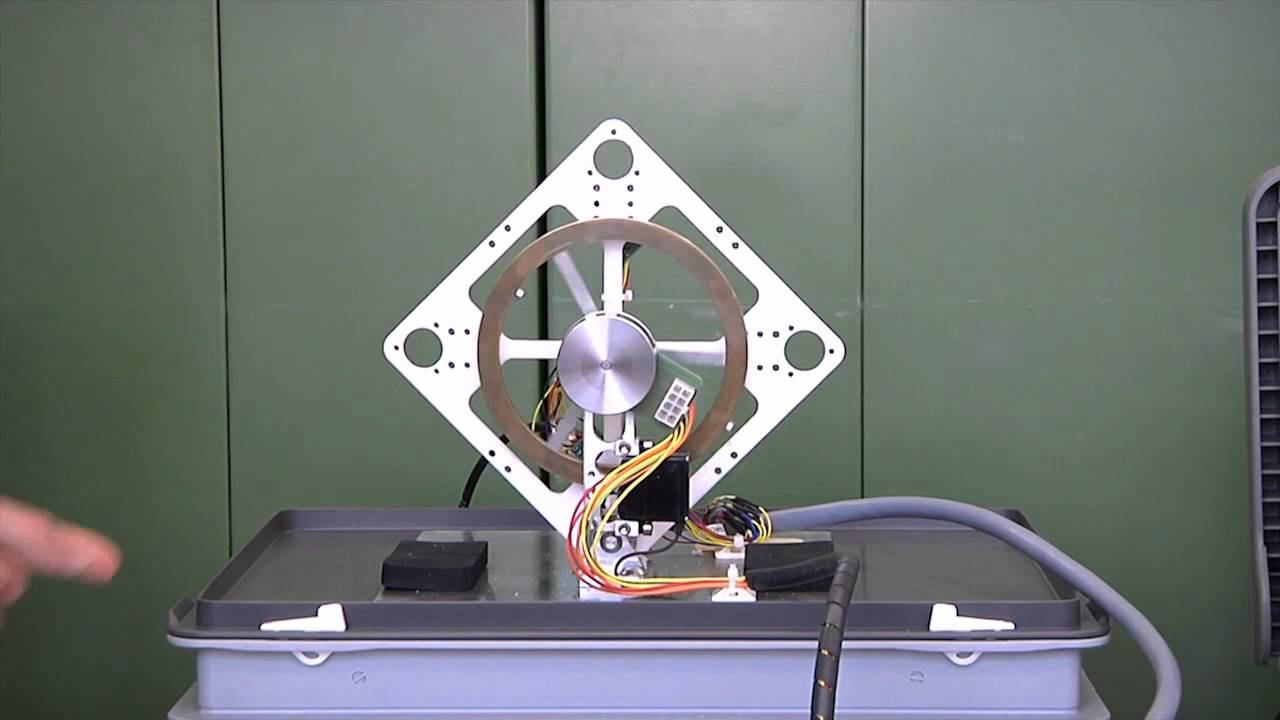
\includegraphics[width=1\textwidth]{images/mechsetup.jpg}
	
	~
	\caption{Possible mechanical setup for the project\cite{cublipic}} 
 	\label{fig:mech} 
\end{figure}

Mechanical pieces of the system:
\begin{itemize}
 \item Aluminium square plate with dimensions of 15x15 cm and holes inside for the reaction wheel mount and to keep the weight low as possible.
 \item Reaction wheel made out of aluminium. Wheel itself is a circle with spokes and a hole in the middle to mount it on the brushless DC motor.
 \item Tabletop mount what can be fixed to one of the corners of the prototype by bearings to have the least amount of friction as possible.
\end{itemize}

This kind of design for the system should be sufficient enough for the aims of the project.